\paragraph{概念}

\begin{itemize}
    \item 割边(桥): 一个无向联通图中, 如果删去边e,该图联通数改变(不再是1),则该边为割边
    \item 边双连通图: 对于一个无向图, 其不拥有割边则为边双连通图
    \item 边双连通分量: 一个无向图的\textbf{极大}边双联通子图被称为边双联通分量
\end{itemize}

\paragraph{性质}

\begin{itemize}
    \item 割边不属于任何边双连通分量, 所以去掉割边后的各个联通子图均是边双连通分量
    \item 对于一个边双中的任意两个点,它们之间都有至少两条\textbf{边不重复}的路径。
\end{itemize}

\paragraph{样例四图片}

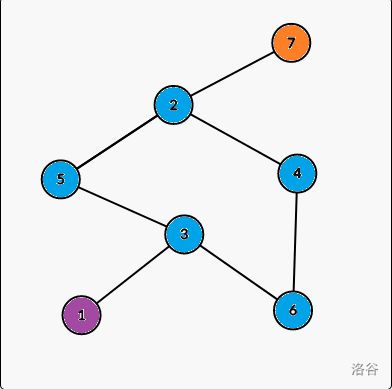
\includegraphics[width=0.4\textwidth]{img/luogu-P8436-1.png}
